% Figure: the knot ladder with its gamma-section cascade, and the Thorin bank for one
% increment. Referenced from §11 before prop:gamma-cascade. Pure TikZ; the plan table's
% "filter bank" figure.

\begin{figure}[t]
\centering
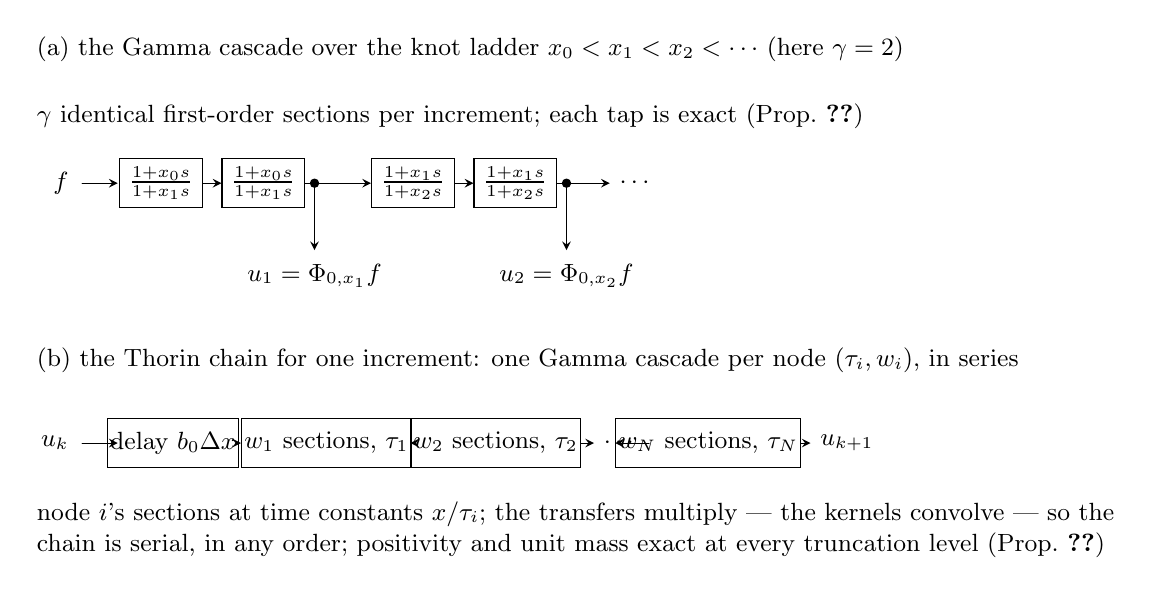
\begin{tikzpicture}[every node/.style={font=\small}, line cap=round, >=stealth,
  sect/.style={draw, minimum width=1.05cm, minimum height=0.62cm, inner sep=1pt},
  tap/.style={fill, circle, inner sep=1.2pt}]

% ---------- panel (a): the gamma-section cascade along the knot ladder ----------
\node[anchor=west] at (-0.3,1.7) {(a) the Gamma cascade over the knot ladder $x_0 < x_1 < x_2 < \cdots$ (here $\gamma = 2$)};
\node[anchor=east] at (0.35,0) {$f$};
\draw[->] (0.4,0) -- (0.85,0);
\node[sect] (a1) at (1.4,0) {$\frac{1+x_0 s}{1+x_1 s}$};
\node[sect] (a2) at (2.7,0) {$\frac{1+x_0 s}{1+x_1 s}$};
\node[sect] (b1) at (4.6,0) {$\frac{1+x_1 s}{1+x_2 s}$};
\node[sect] (b2) at (5.9,0) {$\frac{1+x_1 s}{1+x_2 s}$};
\draw[->] (a1) -- (a2);
\draw[->] (a2) -- (b1);
\draw[->] (b1) -- (b2);
\draw[->] (b2) -- (7.1,0);
\node[anchor=west] at (7.1,0) {$\cdots$};
% taps
\draw[->] (3.35,0) -- (3.35,-0.85); \node[tap] at (3.35,0) {};
\node[anchor=north] at (3.35,-0.9) {$u_1 = \Phi_{0,x_1}f$};
\draw[->] (6.55,0) -- (6.55,-0.85); \node[tap] at (6.55,0) {};
\node[anchor=north] at (6.55,-0.9) {$u_2 = \Phi_{0,x_2}f$};
\node[anchor=west] at (-0.3,0.85) {$\gamma$ identical first-order sections per increment; each tap is exact (Prop.~\ref{prop:knot-exactness})};

% ---------- panel (b): the Thorin chain for one increment ----------
% Redrawn 2026-08-31 (author review): the earlier fan-out/fan-in with a "*" combiner
% read as a parallel bank; the composition is convolution = series connection, so the
% chain is drawn serially, matching panel (a), with the drift's delay block leading.
\begin{scope}[yshift=-3.3cm]
\node[anchor=west] at (-0.3,1.05) {(b) the Thorin chain for one increment: one Gamma cascade per node $(\tau_i, w_i)$, in series};
\node[anchor=east] at (0.35,0) {$u_k$};
\draw[->] (0.4,0) -- (0.85,0);
\node[sect] (d0) at (1.55,0) {delay $b_0\Delta x$};
\node[sect] (t1) at (3.5,0) {$w_1$ sections, $\tau_1$};
\node[sect] (t2) at (5.65,0) {$w_2$ sections, $\tau_2$};
\draw[->] (d0) -- (t1);
\draw[->] (t1) -- (t2);
\draw[->] (t2) -- (6.9,0);
\node[anchor=west] at (6.9,0) {$\cdots$};
\node[sect] (tN) at (8.35,0) {$w_N$ sections, $\tau_N$};
\draw[->] (7.6,0) -- (tN);
\draw[->] (tN) -- (9.65,0);
\node[anchor=west] at (9.65,0) {$u_{k+1}$};
\node[anchor=west] at (-0.3,-0.9) {node $i$'s sections at time constants $x/\tau_i$; the transfers multiply --- the kernels convolve --- so the};
\node[anchor=west] at (-0.3,-1.3) {chain is serial, in any order; positivity and unit mass exact at every truncation level (Prop.~\ref{prop:thorin-subclass})};
\end{scope}

\end{tikzpicture}
\caption{The implementation substrate. (a)~For the Gamma family the increment between
adjacent knots is a cascade of $\gamma$ identical first-order pole--zero sections, and the
record at each knot is read off a tap; the taps are exact for every knot set
(Proposition~\ref{prop:knot-exactness}), so the scale direction is sampled, not
approximated. (b)~For a general Thorin-subclass member the increment is approximated from
inside the axiom class by a serial chain of Gamma cascades, one per atom $(\tau_i, w_i)$ of
the Thorin measure, led by the drift's exact sample delay: the Thorin sum lives in the
exponent, so the transfer functions multiply and the kernels convolve --- a series
connection, in any order --- and every truncation level is itself an admissible family
(Proposition~\ref{prop:thorin-subclass}).}
\label{fig:filterbank}
\end{figure}
